%! Author = chaorn
%! Date = 12.12.24

\begin{frame}{About Me}
    \begin{columns}[T] % Create two columns
        \begin{column}{0.4\textwidth} % Left column: Image or Placeholder
            \centering
            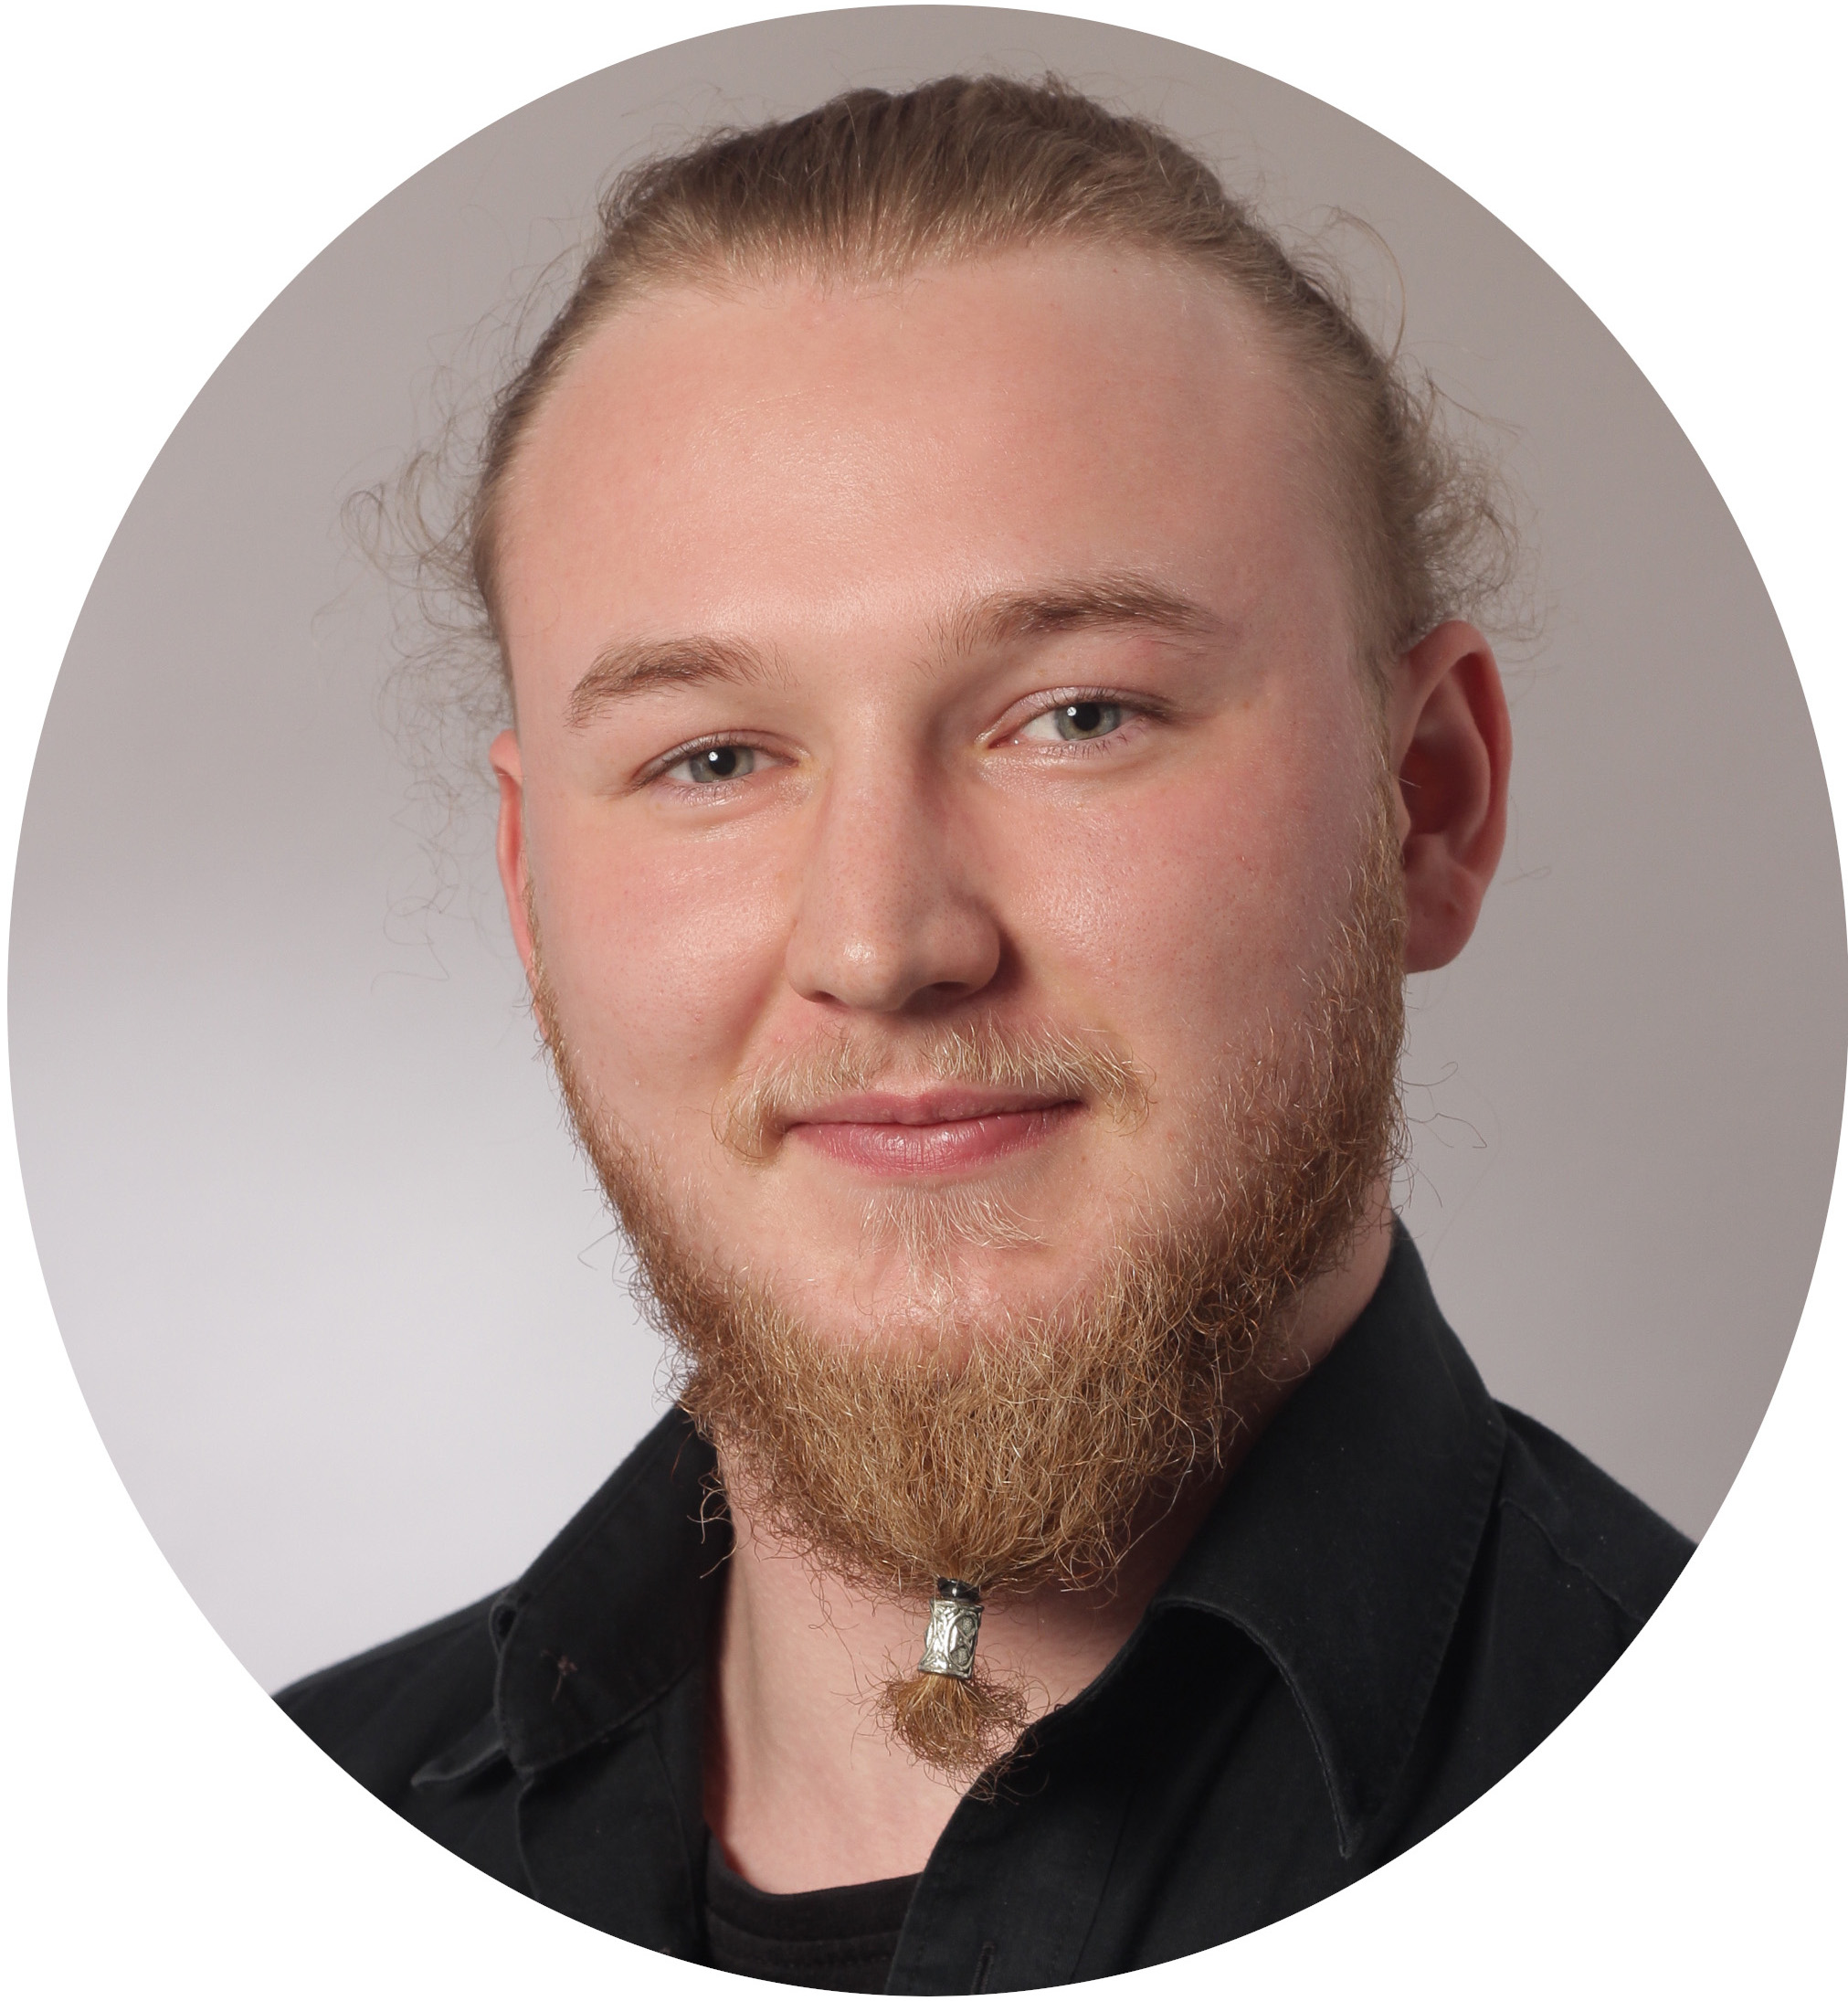
\includegraphics[width=0.8\textwidth]{res/Bewerbungsfoto} % Replace with your image path
            \vspace{0.2cm}
        \end{column}

        \begin{column}{0.6\textwidth} % Right column: Text content
            \textbf{Name:} Sebastian Peschke \\
            \textbf{Ausbildung:} B.Sc. Mobile Computing \\(Hochschule für angewandte Wissenschaften Hof) \\
            \textbf{Kontakt:} \\
            \href{mailto:sebastian.peschke@hof-university.de}{sebastian.peschke@hof-university.de} \\
            \textbf{GitHub:} \\
            \href{https://github.com/ItsMagick}{https://github.com/ItsMagick}
        \end{column}
    \end{columns}
\end{frame}